% !TeX program = xelatex
\documentclass[a4paper,10pt]{article}

% ============================================================================
% កញ្ចប់បណ្ណាល័យ (Packages) – តាមលំនាំស្តង់ដារ អនុវិទ្យាល័យព្រះក្រសាំង (ls_plan.tex)
% បរិបទ៖ ថ្នាក់រៀនគ្មានស្លាយ LCD – បង្រៀនដោយប្រើក្ដារខៀន និងសន្លឹកកិច្ចការសិស្សស-ខ្មៅជាគោល
% ============================================================================
\usepackage[a4paper, left=0.95cm, right=0.95cm, top=0.85cm, bottom=0.92cm, footskip=0.52cm]{geometry}
\usepackage{amsmath}
\usepackage{unicode-math}
\usepackage{fontspec}
\usepackage{array, longtable, multirow, colortbl}
\usepackage[table]{xcolor}
\usepackage{enumitem}
\usepackage{pifont}
\usepackage{fancyhdr}
\usepackage{tikz}
\usetikzlibrary{calc, arrows.meta, angles, quotes, decorations.markings, positioning, babel}

\makeatletter
\let\@expl@@@mark@update@singlecol@structures@@\relax
\makeatother

% ============================================================================
% ការកំណត់ពុម្ពអក្សរផ្លូវការ (Cross-Platform Fonts Configuration)
% ============================================================================
\providecommand{\NGSFindFonts}{%
  \IfFileExists{C:/Windows/Fonts/cambria.ttc}{%
    \def\NGSSysPath{C:/Windows/Fonts/}%
    \def\NGSUserPath{C:/Users/KIT/AppData/Local/Microsoft/Windows/Fonts/}%
  }{%
    \IfFileExists{./fonts/KhmerOSsiemreap.ttf}{\def\NGSSysPath{./fonts/}\def\NGSUserPath{./fonts/}}{%
    \IfFileExists{../fonts/KhmerOSsiemreap.ttf}{\def\NGSSysPath{../fonts/}\def\NGSUserPath{../fonts/}}{%
    \IfFileExists{../../fonts/KhmerOSsiemreap.ttf}{\def\NGSSysPath{../../fonts/}\def\NGSUserPath{../../fonts/}}{%
    \IfFileExists{../../../fonts/KhmerOSsiemreap.ttf}{\def\NGSSysPath{../../../fonts/}\def\NGSUserPath{../../../fonts/}}{%
    \IfFileExists{../../../../fonts/KhmerOSsiemreap.ttf}{\def\NGSSysPath{../../../../fonts/}\def\NGSUserPath{../../../../fonts/}}{%
    \IfFileExists{../../../../../fonts/KhmerOSsiemreap.ttf}{\def\NGSSysPath{../../../../../fonts/}\def\NGSUserPath{../../../../../fonts/}}{%
    \IfFileExists{../../../../../../fonts/KhmerOSsiemreap.ttf}{\def\NGSSysPath{../../../../../../fonts/}\def\NGSUserPath{../../../../../../fonts/}}{%
      \def\NGSSysPath{../../../../../../../fonts/}\def\NGSUserPath{../../../../../../../fonts/}%
    }}}}}}}%
  }%
}
\NGSFindFonts

\setmathfont[Path={\NGSSysPath}, FontIndex=1, Scale=1.02]{cambria.ttc}
\defaultfontfeatures{Ligatures=TeX}

\setmainfont[
  Path={\NGSUserPath},
  Extension=.ttf,
  Script=Khmer,
  BoldFont={KhmerOSsiemreap},
  BoldFeatures={FakeBold=1.8},
  ItalicFont={KhmerOSsiemreap},
  ItalicFeatures={FakeSlant=0.25},
  BoldItalicFont={KhmerOSsiemreap},
  BoldItalicFeatures={FakeBold=1.8, FakeSlant=0.25}
]{KhmerOSsiemreap}

\newfontfamily\muol[Path={\NGSUserPath}, Extension=.ttf, Script=Khmer]{KhmerOSmuollight}
\newfontfamily\TimesEn[Path={\NGSSysPath}, Extension=.ttf, BoldFont={timesbd}, ItalicFont={timesi}, BoldItalicFont={timesbi}]{times}
\newfontfamily\NagaBold[Path={\NGSUserPath}, Extension=.ttf]{AKbalthom Naga Bold}
\newfontfamily\CalibriFont[Path={\NGSSysPath}, Extension=.ttf]{calibri}
\newfontfamily\Tacteing[Path={\NGSUserPath}]{TACTENG.TTF}
\newfontfamily\CourierBullet[Path={\NGSSysPath}, Extension=.ttf]{cour}
\newcommand{\wcirc}{{\CourierBullet\fontsize{9.5pt}{11pt}\selectfont o}}

\XeTeXlinebreaklocale "km"
\XeTeXlinebreakskip = 0pt plus 1pt minus 0.1pt

\definecolor{stepgray}{HTML}{D9D9D9}
\definecolor{headgray}{HTML}{F2F2F2}
\definecolor{boxgray}{HTML}{D9D9D9}
\definecolor{darkred}{HTML}{C00000}
\definecolor{red5e}{HTML}{FF0000}

\pagestyle{fancy}
\fancyhf{}
\renewcommand{\headrulewidth}{0pt}
\fancyfoot[R]{\CalibriFont\fontsize{11pt}{13pt}\selectfont\thepage}

\setlength{\parindent}{0pt}
\setlength{\parskip}{0pt}
\setlength{\tabcolsep}{3.8pt}

\newcolumntype{L}[1]{>{\raggedright\arraybackslash}p{#1}}

\newcommand{\en}[1]{{\TimesEn #1}}
\newcommand{\enbf}[1]{{\TimesEn\textbf{#1}}}
\newcommand{\unit}[1]{\,\text{\en{#1}}}
\newcommand{\fiveE}[1]{{\NagaBold\fontsize{9.5pt}{13pt}\selectfont\textcolor{red5e}{#1}}}
\newcommand{\timenote}[1]{\textcolor{darkred}{\textit{#1}}}
\newcommand{\redsub}[1]{\textcolor{darkred}{#1}}
\newcommand{\graybox}[1]{\colorbox{boxgray}{\strut\hspace{2pt}#1\hspace{2pt}}}
\newcommand{\ditem}{\tikz[baseline=-0.5ex]\fill (0,0.42ex) -- (0.42ex,0) -- (0,-0.42ex) -- (-0.42ex,0) -- cycle;\hspace{0.3em}}
\newcommand{\cnum}[1]{{\fontsize{10.5pt}{12pt}\selectfont\ding{\numexpr171+#1\relax}}\hspace{0.2em}}
\newcommand{\cfig}[1]{\par\vspace{4pt}{\centering #1\par}\vspace{4pt}}
\newcommand{\stepheader}[1]{\multicolumn{3}{|c|}{\cellcolor{stepgray}\muol #1} \\* \noalign{\hrule height 0.4pt}}
\newcommand{\tri}[1]{\ensuremath{\triangle #1}}
\newcommand{\ang}[1]{\ensuremath{\angle #1}}
\newcommand{\cg}{\ensuremath{\cong}}
\newcommand{\khmflourish}{{\Tacteing\fontsize{36pt}{14pt}\selectfont\raisebox{-5pt}{3}}}

\tikzset{
  tk1/.style={postaction={decorate},decoration={markings,mark=at position 0.50 with {\draw[black, line width=0.85pt](0,-0.095)--(0,0.095);}}},
  tk2/.style={postaction={decorate},decoration={markings,
    mark=at position 0.45 with {\draw[black, line width=0.85pt](0,-0.095)--(0,0.095);},
    mark=at position 0.55 with {\draw[black, line width=0.85pt](0,-0.095)--(0,0.095);}}},
  tk3/.style={postaction={decorate},decoration={markings,
    mark=at position 0.42 with {\draw[black, line width=0.85pt](0,-0.095)--(0,0.095);},
    mark=at position 0.50 with {\draw[black, line width=0.85pt](0,-0.095)--(0,0.095);},
    mark=at position 0.58 with {\draw[black, line width=0.85pt](0,-0.095)--(0,0.095);}}},
  par1/.style={postaction={decorate},decoration={markings,mark=at position 0.52 with {\draw[black, line width=0.85pt](-0.07,0.08)--(0.05,0)--(-0.07,-0.08);}}}
}

% ============================================================================
% ម៉ាក្រូរូបភាពធរណីមាត្រស-ខ្មៅ (Proportional 4.2–7.2 cm B&W TikZ Diagrams)
% ============================================================================

% ១. រំលឹកមេរៀនទាក់ទង៖ ចតុកោណកែង + ចតុកោណស្មើ => ការេ (Square)
\newcommand{\figPrereqSQ}{%
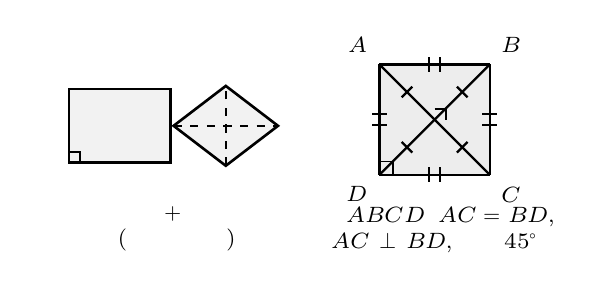
\begin{tikzpicture}[scale=0.78, every node/.style={font=\footnotesize, text=black}]
  % ឆ្វេង៖ ចតុកោណកែង + ចតុកោណស្មើ
  \begin{scope}[shift={(0,0)}]
    \draw[black, line width=0.95pt, fill=gray!10] (0,0.20) rectangle (1.65,1.40);
    \draw[black, line width=0.65pt] (0,0.38)--(0.18,0.38)--(0.18,0.20);
    \node[font=\bfseries] at (2.12,0.80) {$+$};
    \begin{scope}[shift={(2.55,0.80)}]
      \draw[black, line width=0.95pt, fill=gray!10] (-0.85,0)--(0,0.65)--(0.85,0)--(0,-0.65)--cycle;
      \draw[black, line width=0.7pt, dashed] (-0.85,0)--(0.85,0) (0,-0.65)--(0,0.65);
    \end{scope}
    \node[anchor=north, text width=3.55cm, align=center] at (1.75,-0.35) {ចតុកោណកែង $+$ ចតុកោណស្មើ\\(រួមលក្ខណៈទាំងអស់)};
  \end{scope}
  % ស្ដាំ៖ ការេ ABCD
  \begin{scope}[shift={(5.05,0)}]
    \coordinate (D) at (0,0); \coordinate (C) at (1.80,0);
    \coordinate (A) at (0,1.80); \coordinate (B) at (1.80,1.80);
    \coordinate (O) at (0.90,0.90);
    \fill[gray!14] (A)--(B)--(C)--(D)--cycle;
    \draw[black, line width=1.0pt, tk2] (A)--(B); \draw[black, line width=1.0pt, tk2] (B)--(C);
    \draw[black, line width=1.0pt, tk2] (C)--(D); \draw[black, line width=1.0pt, tk2] (D)--(A);
    \draw[black, line width=0.85pt, tk1] (A)--(O); \draw[black, line width=0.85pt, tk1] (O)--(C);
    \draw[black, line width=0.85pt, tk1] (B)--(O); \draw[black, line width=0.85pt, tk1] (O)--(D);
    \draw[black, line width=0.65pt] (0,0.22)--(0.22,0.22)--(0.22,0);
    \draw[black, line width=0.65pt] (0.90,1.08)--(1.08,1.08)--(1.08,0.90);
    \node[above left=1pt] at (A) {$A$}; \node[above right=1pt] at (B) {$B$};
    \node[below right=1pt] at (C) {$C$}; \node[below left=1pt] at (D) {$D$};
    \node[anchor=north, text width=3.25cm, align=center] at (0.90,-0.35) {ការេ $ABCD$៖ $AC=BD$,\\$AC\perp BD$, មុំពុះ $45^\circ$};
  \end{scope}
\end{tikzpicture}}

% ២. E1 Engage: វាស់ទទឹងបឹង BC តាមបាតមធ្យម DE និងធ្នឹមដំបូលកែង BO = 1/2 AC
\newcommand{\figEngageSQ}{%
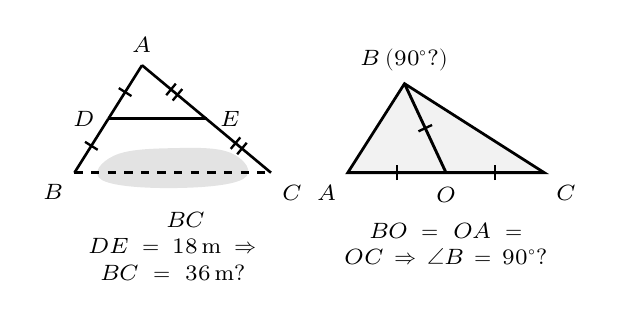
\begin{tikzpicture}[scale=0.78, every node/.style={font=\footnotesize, text=black}]
  % ឆ្វេង៖ វាស់ទទឹងបឹង BC តាមបាតមធ្យម DE
  \begin{scope}[shift={(0,0)}]
    \coordinate (B) at (0,0); \coordinate (C) at (3.20,0);
    \coordinate (A) at (1.10,1.75);
    \coordinate (D) at ($(A)!0.5!(B)$); \coordinate (E) at ($(A)!0.5!(C)$);
    % បឹងទឹកចន្លោះ B និង C
    \fill[gray!22] plot[smooth cycle, tension=0.7] coordinates {(0.45,-0.12) (1.60,-0.25) (2.75,-0.10) (2.55,0.32) (1.60,0.40) (0.65,0.28)};
    \draw[black, line width=1.0pt, dashed] (B)--(C);
    \draw[black, line width=0.95pt, tk1] (A)--(D); \draw[black, line width=0.95pt, tk1] (D)--(B);
    \draw[black, line width=0.95pt, tk2] (A)--(E); \draw[black, line width=0.95pt, tk2] (E)--(C);
    \draw[black, line width=1.1pt] (D)--(E);
    \node[above=1pt] at (A) {$A$}; \node[below left=1pt] at (B) {$B$}; \node[below right=1pt] at (C) {$C$};
    \node[left=1.5pt] at (D) {$D$}; \node[right=1.5pt] at (E) {$E$};
    \node[anchor=north, text width=3.45cm, align=center] at (1.60,-0.48) {វាស់ទទឹងបឹង $BC$ ដោយវាស់\\$DE=18\unit{m} \Rightarrow BC=36\unit{m}$?};
  \end{scope}
  % ស្ដាំ៖ ធ្នឹមដំបូលកែង BO = OA = OC
  \begin{scope}[shift={(4.45,0)}]
    \coordinate (A) at (0,0); \coordinate (C) at (3.20,0);
    \coordinate (O) at (1.60,0);
    \coordinate (B) at ({1.60 + 1.60*cos(115)}, {1.60*sin(115)});
    \fill[gray!10] (A)--(B)--(C)--cycle;
    \draw[black, line width=1.0pt] (A)--(B)--(C)--cycle;
    \draw[black, line width=1.0pt, tk1] (A)--(O);
    \draw[black, line width=1.0pt, tk1] (O)--(C);
    \draw[black, line width=1.05pt, tk1] (B)--(O);
    \node[above=1pt] at (B) {$B\;(90^\circ?)$};
    \node[below left=1pt] at (A) {$A$}; \node[below=1.5pt] at (O) {$O$}; \node[below right=1pt] at (C) {$C$};
    \node[anchor=north, text width=3.45cm, align=center] at (1.60,-0.48) {ធ្នឹមដំបូល៖ ដាក់ជន្ទល់\\$BO=OA=OC \Rightarrow \ang{B}=90^\circ$?};
  \end{scope}
\end{tikzpicture}}

% ៣. E2/E3: គន្លឹះ Polya បន្លាយអង្កត់ទ្វេដង (DE=EF បង្កើតប្រលេឡូក្រាម & BO=OD បង្កើតចតុកោណកែង)
\newcommand{\figPolyaSQ}{%
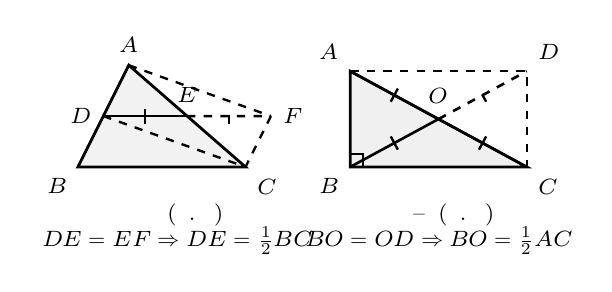
\begin{tikzpicture}[scale=0.76, every node/.style={font=\footnotesize, text=black}]
  % ឆ្វេង៖ រូបសៀវភៅគោល ទំ.១៨០ (បន្លាយ DE=EF => ADCF & BDFC ប្រលេឡូក្រាម)
  \begin{scope}[shift={(0,0)}]
    \coordinate (B) at (0,0); \coordinate (C) at (2.80,0);
    \coordinate (A) at (0.85,1.70);
    \coordinate (D) at ($(A)!0.5!(B)$); \coordinate (E) at ($(A)!0.5!(C)$);
    \coordinate (F) at ($(E)!-1!(D)$);
    \fill[gray!10] (A)--(B)--(C)--cycle;
    \draw[black, line width=1.0pt] (A)--(B)--(C)--cycle;
    \draw[black, line width=1.0pt, tk1] (D)--(E);
    \draw[black, line width=0.95pt, dashed, tk1] (E)--(F);
    \draw[black, line width=0.85pt, dashed] (A)--(F) (F)--(C) (D)--(C);
    \node[above=1pt] at (A) {$A$}; \node[below left=1pt] at (B) {$B$}; \node[below right=1pt] at (C) {$C$};
    \node[left=1pt] at (D) {$D$}; \node[above=1.5pt] at (E) {$E$}; \node[right=1pt] at (F) {$F$};
    \node[anchor=north, text width=3.55cm, align=center] at (1.65,-0.45) {ទ្រឹស្ដីបទទី១ (ទំ.១៨០)៖ បន្លាយ\\$DE=EF \Rightarrow DE=\frac{1}{2}BC$};
  \end{scope}
  % ស្ដាំ៖ រូបសៀវភៅគោល ទំ.១៨១ (បន្លាយ BO=OD => ABCD ចតុកោណកែង)
  \begin{scope}[shift={(4.55,0)}]
    \coordinate (B) at (0,0); \coordinate (C) at (2.95,0);
    \coordinate (A) at (0,1.60); \coordinate (D) at (2.95,1.60);
    \coordinate (O) at (1.475,0.80);
    \fill[gray!12] (A)--(B)--(C)--cycle;
    \draw[black, line width=1.0pt] (A)--(B)--(C)--cycle;
    \draw[black, line width=0.85pt, dashed] (A)--(D)--(C);
    \draw[black, line width=0.95pt, tk1] (B)--(O);
    \draw[black, line width=0.95pt, dashed, tk1] (O)--(D);
    \draw[black, line width=0.9pt, tk1] (A)--(O); \draw[black, line width=0.9pt, tk1] (O)--(C);
    \draw[black, line width=0.7pt] (0,0.22)--(0.22,0.22)--(0.22,0);
    \node[above left=1pt] at (A) {$A$}; \node[below left=1pt] at (B) {$B$};
    \node[below right=1pt] at (C) {$C$}; \node[above right=1pt] at (D) {$D$};
    \node[above=2pt] at (O) {$O$};
    \node[anchor=north, text width=3.45cm, align=center] at (1.48,-0.45) {ទ្រឹស្ដីបទទី៣--៤ (ទំ.១៨១)៖ បន្លាយ\\$BO=OD \Rightarrow BO=\frac{1}{2}AC$};
  \end{scope}
\end{tikzpicture}}

% ៤. E4 Elaborate: គំរូទី១ (លំ.៨ ទំ.១៨៦៖ DE=9x-4, BC=6x+4) & គំរូទី២ (មេដ្យាន BO=6.5 & ការេ MNPQ)
\newcommand{\figModelSQ}{%
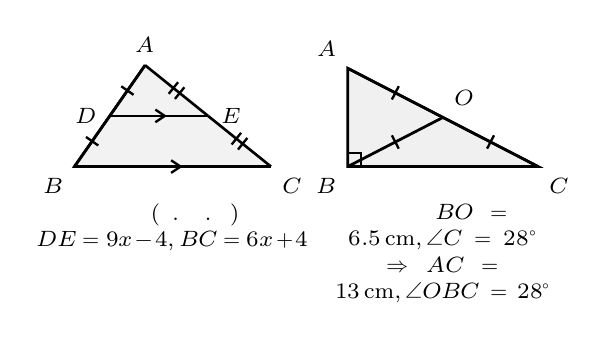
\begin{tikzpicture}[scale=0.78, every node/.style={font=\footnotesize, text=black}]
  % ឆ្វេង៖ លំហាត់ទី៨ ទំ.១៨៦
  \begin{scope}[shift={(0,0)}]
    \coordinate (B) at (0,0); \coordinate (C) at (3.20,0);
    \coordinate (A) at (1.15,1.65);
    \coordinate (D) at ($(A)!0.5!(B)$); \coordinate (E) at ($(A)!0.5!(C)$);
    \fill[gray!10] (A)--(B)--(C)--cycle;
    \draw[black, line width=1.0pt] (A)--(B)--(C);
    \draw[black, line width=0.95pt, tk1] (A)--(D); \draw[black, line width=0.95pt, tk1] (D)--(B);
    \draw[black, line width=0.95pt, tk2] (A)--(E); \draw[black, line width=0.95pt, tk2] (E)--(C);
    \draw[black, line width=1.0pt, par1] (D)--(E); \draw[black, line width=1.0pt, par1] (B)--(C);
    \node[above=1pt] at (A) {$A$}; \node[below left=1pt] at (B) {$B$}; \node[below right=1pt] at (C) {$C$};
    \node[left=1.5pt] at (D) {$D$}; \node[right=1.5pt] at (E) {$E$};
    \node[anchor=north, text width=3.45cm, align=center] at (1.60,-0.45) {គំរូទី១ (លំ.៨ ទំ.១៨៦)៖\\$DE=9x-4, BC=6x+4$};
  \end{scope}
  % ស្ដាំ៖ គំរូទី២ (ត្រីកោណកែង ABC មេដ្យាន BO=6.5cm)
  \begin{scope}[shift={(4.45,0)}]
    \coordinate (B) at (0,0); \coordinate (C) at (3.10,0);
    \coordinate (A) at (0,1.60); \coordinate (O) at (1.55,0.80);
    \fill[gray!12] (A)--(B)--(C)--cycle;
    \draw[black, line width=1.0pt] (A)--(B)--(C)--cycle;
    \draw[black, line width=0.95pt, tk1] (A)--(O);
    \draw[black, line width=0.95pt, tk1] (O)--(C);
    \draw[black, line width=1.0pt, tk1] (B)--(O);
    \draw[black, line width=0.7pt] (0,0.22)--(0.22,0.22)--(0.22,0);
    \node[above left=1pt] at (A) {$A$}; \node[below left=1pt] at (B) {$B$};
    \node[below right=1pt] at (C) {$C$}; \node[above right=1pt] at (O) {$O$};
    \node[anchor=north, text width=3.45cm, align=center] at (1.55,-0.45) {គំរូទី២៖ $BO=6.5\unit{cm}, \ang{C}=28^\circ$\\$\Rightarrow AC=13\unit{cm}, \ang{OBC}=28^\circ$};
  \end{scope}
\end{tikzpicture}}

% ៥. E5 Evaluate: ត្រីកោណបាតមធ្យម \triangle DEF ក្នុង \triangle ABC
\newcommand{\figPractSQ}{%
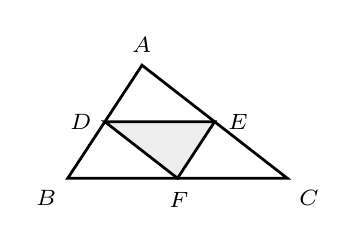
\begin{tikzpicture}[scale=0.82, every node/.style={font=\footnotesize, text=black}]
  \coordinate (B) at (0,0); \coordinate (C) at (3.40,0);
  \coordinate (A) at (1.15,1.75);
  \coordinate (D) at ($(A)!0.5!(B)$);
  \coordinate (E) at ($(A)!0.5!(C)$);
  \coordinate (F) at ($(B)!0.5!(C)$);
  \fill[gray!14] (D)--(E)--(F)--cycle;
  \draw[black, line width=1.0pt] (A)--(B)--(C)--cycle;
  \draw[black, line width=1.0pt] (D)--(E)--(F)--cycle;
  \node[above=1pt] at (A) {$A$}; \node[below left=1pt] at (B) {$B$}; \node[below right=1pt] at (C) {$C$};
  \node[left=1.5pt] at (D) {$D$}; \node[right=1.5pt] at (E) {$E$}; \node[below=1.5pt] at (F) {$F$};
\end{tikzpicture}}

\begin{document}
\fontsize{10pt}{15.2pt}\selectfont

% -------------------- ក្បាលកិច្ចតែងការ (Header) --------------------
\begin{center}
  {\muol\fontsize{11pt}{16pt}\selectfont ព្រះរាជាណាចក្រកម្ពុជា}\\[2pt]
  {\muol\fontsize{10pt}{15pt}\selectfont ជាតិ សាសនា ព្រះមហាក្សត្រ}\\[1pt]
  \khmflourish
\end{center}

\vspace{-28pt}
{\muol\fontsize{9.5pt}{12.5pt}\selectfont
មន្ទីរអប់រំ យុវជន និងកីឡា ខេត្តកំពង់ធំ\\
ការិយាល័យអប់រំ យុវជន និងកីឡា ស្រុកកំពង់ស្វាយ\\
អនុវិទ្យាល័យព្រះក្រសាំង}

\vspace{1pt}
\begin{center}
  {\muol\fontsize{10pt}{14pt}\selectfont កិច្ចតែងការបង្រៀន}
\end{center}
\vspace{0pt}

% -------------------- ព័ត៌មានទូទៅ (Metadata) --------------------
{\renewcommand{\arraystretch}{0.95}
\hspace*{4.05cm}%
\begin{tabular}{@{}l l l@{}}
  - \hspace{0.35cm} មុខវិជ្ជា & : & គណិតវិទ្យា ថ្នាក់ទី៨ \\
  - \hspace{0.35cm} ចំណងជើងមេរៀន & : & មេរៀនទី១៣ ចតុកោណ \\
  - \hspace{0.35cm} ចំណងជើងរង & : & ២.៤ លក្ខណៈការេ និងទ្រឹស្ដីបទចំណុចកណ្ដាល (ទំ.១៧៩--១៨១, ១៨៦) \\
  - \hspace{0.35cm} រយៈពេល & : & ១ ម៉ោងសិក្សា (៥០ នាទី) \\
  - \hspace{0.35cm} បង្រៀនដោយ & : & ហុក ប៊ុនថែន \\
  - \hspace{0.35cm} កាលបរិច្ឆេទ & : & ថ្ងៃព្រហស្បតិ៍ ៨កើត ខែមិគសិរ ព.ស.២៥៧០ (១៧ ធ្នូ ២០២៦) \\
\end{tabular}

\vspace{1pt}

% -------------------- I. វត្ថុបំណង --------------------
\textbf{I.} {\muol វត្ថុបំណង}\\[1pt]
\hspace*{0.55cm}%
\begin{tabular}{@{}l l L{14.2cm}@{}}
  \wcirc \hspace{0.25cm} វិជ្ជាសម្បទា & : & សិស្សពោលបានត្រឹមត្រូវនូវនិយមន័យ និងលក្ខណៈទាំង ៧ នៃការេ ព្រមទាំងទ្រឹស្ដីបទចំណុចកណ្ដាលទាំង ៤៖ ទ្រឹស្ដីបទទី១--២ (បាតមធ្យមនៃត្រីកោណ $DE\parallel BC, DE=\frac{1}{2}BC$ និងច្រាស) និងទ្រឹស្ដីបទទី៣--៤ (មេដ្យានត្រីកោណកែងចំពោះអ៊ីប៉ូតេនុស $BO=\frac{1}{2}AC$ និងច្រាស) តាមសៀវភៅគោល ទំ.១៧៩--១៨១ ។ \\
  \wcirc \hspace{0.25cm} បំណិនសម្បទា & : & សិស្សប្រើគន្លឹះសង់បន្លាយអង្កត់ទ្វេដង ($DE=EF$ និង $BO=OD$) ដើម្បីស្រាយបញ្ជាក់ទ្រឹស្ដីបទលើសន្លឹកកិច្ចការស-ខ្មៅ និងដោះស្រាយលំហាត់គណនាប្រវែងបាតមធ្យម មេដ្យានត្រីកោណកែង និងអង្កត់ទ្រូងការេដោយភ្ជាប់ហេតុផល \cnum{1}--\cnum{5} ។ \\
  \wcirc \hspace{0.25cm} ចរិយាសម្បទា & : & សិស្សមានទម្លាប់ពិនិត្យលក្ខខណ្ឌចំណុចកណ្ដាល និងមុំកែងមុនប្រើរូបមន្ត $\frac{1}{2}$ ព្រមទាំងឃើញតម្លៃអនុវត្តជាក់ស្ដែងក្នុងការវាស់ចម្ងាយឆ្លងឧបសគ្គ និងការផ្សារគ្រោងដំបូលកែង ។ \\
\end{tabular}

\vspace{1pt}

% -------------------- II. សម្ភារៈឧបទេស --------------------
\textbf{II.} {\muol សម្ភារៈឧបទេស}\\[1pt]
\hspace*{0.55cm}$\bullet$ \hspace{0.35cm} សៀវភៅសិក្សាគោលគណិតវិទ្យាថ្នាក់ទី៨ (ទំ.១៧៩--១៨១ និង ១៨៥--១៨៦) ក្ដារខៀន ដីស បន្ទាត់ក្រិត រ៉ាប់ព័រទ័រ ដែកឈាន និងសន្លឹកកិច្ចការសិស្សស-ខ្មៅ (\en{Worksheet\_SQMID1} ចំនួន ២ ទំព័រ \en{A4} ដោយគ្មានស្លាយ \en{LCD}) ។

\vspace{1pt}

% -------------------- III. វិធីសាស្រ្តបង្រៀន --------------------
\textbf{III.} {\muol វិធីសាស្រ្តបង្រៀន}\\[1pt]
\hspace*{0.45cm}%
\begin{tabular}{@{}l l L{14.85cm}@{}}
  $\bullet$ \hspace{0.25cm} គោលវិធី & : & សិស្សមជ្ឈមណ្ឌល (សិក្សាស៊ើបអង្កេតជាដៃគូលើសន្លឹកកិច្ចការបំពេញផ្ទាល់ គ្មានស្លាយ \en{LCD}) \\
  $\bullet$ \hspace{0.25cm} យុទ្ធវិធីបង្រៀន & : & គម្រូស្ថាបនានិយម \en{5Es} រួមបញ្ចូល \textbf{វិធីសង់បន្លាយអង្កត់ទ្វេដងបង្កើតប្រលេឡូក្រាម និងចតុកោណកែងរបស់ Polya} (\en{Polya Auxiliary Segment-Doubling — Polya, 1945; Palatnik \& Sigler, 2019}) \\
\end{tabular}
}

\vspace{1pt}

% -------------------- IV. ដំណើរការបង្រៀន --------------------
\textbf{IV.} {\muol ដំណើរការបង្រៀន}

\vspace{1pt}

\renewcommand{\arraystretch}{1.15}
\begin{longtable}{|L{5.50cm}|L{7.90cm}|L{4.80cm}|}
\hline
\rowcolor{headgray}
\multicolumn{1}{|c|}{\muol សកម្មភាពគ្រូ} &
\multicolumn{1}{c|}{\muol ខ្លឹមសារមេរៀន} &
\multicolumn{1}{c|}{\muol សកម្មភាពសិស្ស} \\
\hline
\endhead
\hline
\endfoot
\hline
\endlastfoot

% ==================== ជំហានទី១ (2min) ====================
\stepheader{ជំហានទី១ \enbf{(}រដ្ឋបាលថ្នាក់\enbf{)}}
$\bullet$ ពិនិត្យអវត្តមាន សណ្ដាប់ធ្នាប់ អនាម័យ និងសម្ភារៈធរណីមាត្រ (បន្ទាត់ក្រិត រ៉ាប់ព័រទ័រ ដែកឈាន)
&
$\bullet$ ពិនិត្យវត្តមាន និងសណ្ដាប់ធ្នាប់ថ្នាក់រៀន \par
$\bullet$ ត្រៀមបន្ទាត់ក្រិត រ៉ាប់ព័រទ័រ និងដែកឈាន
&
$\circ$ ប្រធានថ្នាក់រាយការណ៍អវត្តមាន និងត្រៀមឧបករណ៍ធរណីមាត្រ \\[3pt]

$\bullet$ រៀបចំសិស្សជាដៃគូពិភាក្សា រួចចែកសន្លឹកកិច្ចការ \en{Worksheet\_SQMID1} (២ ទំព័រ \en{A4}) ផ្កាប់លើតុ
&
$\bullet$ ការចាត់ដៃគូសិក្សា និងចែកសន្លឹកកិច្ចការស-ខ្មៅ
&
$\circ$ អង្គុយតាមដៃគូ និងទទួលសន្លឹកកិច្ចការទុកលើតុ \\
\hline

% ==================== ជំហានទី២ (9min: <=3 + 3 + E1 3) ====================
\stepheader{ជំហានទី២ \enbf{(}កិច្ចការផ្ទះ \enbf{+} ទំនាក់ទំនងមេរៀនថ្មី\enbf{)}}
\ditem \textbf{កំណែកិច្ចការផ្ទះ ($\le 3\unit{min}$)} \timenote{សង្ខេបខ្លីលើក្ដារខៀន}
&
{\centering\redsub{កំណែកិច្ចការផ្ទះ (លំហាត់ទី១, ទី១៣ និងទី១៤ ទំ.១៨៥--១៨៦)}\par}
&
$\circ$ យកសៀវភៅកិច្ចការផ្ទះមកផ្ទៀងផ្ទាត់ \\[2pt]

$\bullet$ ផ្ទៀងផ្ទាត់ការសង់ចតុកោណស្មើ និងចម្លើយលំហាត់ទី១៣--១៤ លើក្ដារខៀន
&
$\bullet$ \textbf{លំ.១៖} គូស $AC=5\unit{cm}\perp BD=8\unit{cm}$ កាត់ពាក់កណ្ដាលគ្នាត្រង់ $O$ ($2.5\unit{cm}$ និង $4\unit{cm}$) ។ \par
$\bullet$ \textbf{លំ.១៣--១៤៖} $\tri{ABE}\cg\tri{CDF}\Rightarrow BE=DF$; ក្នុង $\tri{OCD}$ កែងត្រង់ $O$ គេបាន $\ang{ODC}+\ang{OCD}=90^\circ$ ។
&
$\circ$ ផ្ទៀងផ្ទាត់ចម្លើយ និងកែលម្អចំណុចខ្វះខាត \\[3pt]

\ditem \textbf{រំលឹកមេរៀនទាក់ទង ($3\unit{min}$)} \par
$\bullet$ គូសរូបលើក្ដារខៀន សួររំលឹក៖ «បើប្រលេឡូក្រាមមួយជា\textbf{ចតុកោណកែងផង} និងជា\textbf{ចតុកោណស្មើផង} តើវាជាចតុកោណអ្វី? ហើយអង្កត់ទ្រូងវាមានលក្ខណៈដូចម្ដេច?»
&
{\centering\redsub{រំលឹកមេរៀនទាក់ទងមេរៀនថ្មី}\par} \par
$\bullet$ \textbf{ការេ} ជាចតុកោណស្មើមានមុំកែងមួយ (ឬចតុកោណកែងមានជ្រុងជាប់ស្មើគ្នា) ។ \par
$\bullet$ អង្កត់ទ្រូងការេ៖ \textbf{ប៉ុនគ្នា} ($AC=BD$), \textbf{កែងគ្នា} ($AC\perp BD$) ត្រង់ចំណុចកណ្ដាល $O$ និង\textbf{ពុះមុំកែងជា $45^\circ$}!
&
$\circ$ ឆ្លើយផ្ទាល់មាត់៖ «ជាការេ! អង្កត់ទ្រូងទាំងប៉ុនគ្នា ទាំងកែងគ្នា ទាំងពុះមុំជា $45^\circ$!» \\[3pt]

&
\cfig{\figPrereqSQ}
& \\[3pt]

\fiveE{E1 - Engage (3min)} \timenote{(កុំទាន់ផ្ដល់ចម្លើយ)} \par
\ditem \textbf{បញ្ហាភ្ញាក់ផ្អើល «វាស់ទទឹងបឹងដោយមិនឆ្លងទឹក និងជន្ទល់ដំបូលកែង»៖} \par
$\bullet$ លើកស្ថានភាពជាក់ស្ដែងទាំងពីរលើក្ដារខៀន (មានរូបលើសន្លឹកកិច្ចការផ្នែកទី១)
&
{\centering\redsub{ស្ថានភាពបញ្ហា៖ ទទឹងបឹង និងជន្ទល់ដំបូលកែង}\par}
&
$\circ$ សង្កេតរូបស្ថានភាពទាំងពីរលើក្ដារខៀន និងលើសន្លឹកកិច្ចការ \\[3pt]

&
\cfig{\figEngageSQ}
& \\[3pt]

– \textbf{សំណួរបំផុស៖} «(១) ហេតុអ្វីគ្រាន់តែវាស់អង្កត់ភ្ជាប់ចំណុចកណ្ដាល $DE=18\unit{m}$ លើគោក ដឹងភ្លាមថាទទឹងបឹង $BC=36\unit{m}$? (២) ហេតុអ្វីជាងដែកដាក់ជន្ទល់កណ្ដាល $BO=OA=OC$ ធ្វើឱ្យមុំកំពូលដំបូល $\ang{B}=90^\circ$ គត់?»
&
\textbf{ចម្ងល់គោលប្រចាំម៉ោង៖} \par
តើអាចប្រើគំនិតរួមតែមួយ (សង់បន្លាយអង្កត់ទ្វេដងបង្កើតប្រលេឡូក្រាម និងចតុកោណកែង) ដើម្បីស្រាយបញ្ជាក់រូបមន្ត «ពាក់កណ្ដាល ($\frac{1}{2}$)» ទាំងពីរនេះដោយរបៀបណា?
&
$\circ$ ពិភាក្សាជាដៃគូ ៣០ វិនាទី និងគូសធីកការទស្សន៍ទាយដំបូងក្នុងប្រអប់ \en{E1} លើសន្លឹកកិច្ចការ \\
\hline

% ==================== ជំហានទី៣ (17min: E2 11m + E3 6m) ====================
\stepheader{ជំហានទី៣ \enbf{(}ខ្លឹមសារមេរៀនថ្មី\enbf{)}}
\fiveE{E2 - Explore (11min)} \par
$\bullet$ សរសេរចំណងជើងរងលើក្ដារខៀន និងឱ្យសិស្សបើកសន្លឹកកិច្ចការទំព័រទី១ ផ្នែកទី២
&
២.៤ លក្ខណៈការេ និងទ្រឹស្ដីបទចំណុចកណ្ដាល (ទំ.១៧៩--១៨១)
&
$\circ$ កត់ចំណងជើងរងចូលសៀវភៅសរសេរ និងបើកសន្លឹកកិច្ចការទំព័រទី១ \\[3pt]

\ditem \textbf{សកម្មភាពទី១៖ វាស់ផ្ទៀងផ្ទាត់ខ្នាតពិត 1:1 លើសន្លឹកកិច្ចការ ($4\unit{min}$)} \par
$\bullet$ ឱ្យដៃគូសិស្សប្រើបន្ទាត់ក្រិតវាស់រូបខ្នាតពិតលើសន្លឹកកិច្ចការ៖ (១) បាតមធ្យម $DE$ ធៀបនឹងជ្រុង $BC=4.4\unit{cm}$ និង (២) មេដ្យាន $QO$ ធៀបនឹងអ៊ីប៉ូតេនុស $PR=4.0\unit{cm}$ នៃត្រីកោណកែង $\tri{PQR}$!
&
{\centering\textbf{លទ្ធផលពិសោធន៍វាស់ខ្នាតពិត 1:1}\par} \par
$\bullet$ ក្នុង $\tri{ABC}$ ($D,E$ ចំណុចកណ្ដាល)៖ $DE = 2.2\unit{cm} = \frac{1}{2}BC$ ហើយ $DE\parallel BC$! \par
$\bullet$ ក្នុងត្រីកោណកែង $\tri{PQR}$ ($\ang{Q}=90^\circ$)៖ មេដ្យាន $QO = 2.0\unit{cm} = \frac{1}{2}PR$ (\graybox{$QO=OP=OR$})!
&
$\circ$ វាស់ប្រវែងជាក់ស្ដែងលើសន្លឹកកិច្ចការ និងសង្កេតឃើញទំនាក់ទំនង $\frac{1}{2}$ ទាំងពីរ \\[3pt]

\ditem \textbf{សកម្មភាពទី២៖ គន្លឹះ Polya «បន្លាយអង្កត់ទ្វេដង» ស្រាយបញ្ជាក់ទ្រឹស្ដីបទ ($7\unit{min}$)} \par
$\bullet$ ណែនាំគន្លឹះមាស \en{Polya}៖ «ឃើញ $\frac{1}{2}$ ឱ្យបន្លាយអង្កត់នោះទ្វេដង!» រួចដឹកនាំសិស្សបំពេញ \textbf{ផ្នែក ក (ទ្រឹស្ដីបទទី១ ទំ.១៨០៖ បន្លាយ $DE=EF$)}
&
\textbf{ការស្រាយបញ្ជាក់ដោយបន្លាយអង្កត់ទ្វេដង (\en{Polya})៖} \par
$\bullet$ \textbf{ផ្នែក ក (បាតមធ្យមត្រីកោណ)៖} បន្លាយ $DE$ ឱ្យបាន $DE=EF$ នោះ $ADCF$ មានអង្កត់ទ្រូងកាត់ពាក់កណ្ដាលគ្នាត្រង់ $E$ ជាប្រលេឡូក្រាម $\Rightarrow AD=CF, AB\parallel CF$ ។ ដោយ $AD=DB$ គេបាន $DB=CF, DB\parallel CF \Rightarrow BDFC$ ជាប្រលេឡូក្រាម $\Rightarrow DE\parallel BC$ និង $DE=\frac{1}{2}DF=\frac{1}{2}BC$!
&
$\circ$ គូសបន្ទាត់ដាច់ៗបន្លាយ $DE=EF$ និងបំពេញសម្រាយបញ្ជាក់ \textbf{ផ្នែក ក} \\[2pt]

$\bullet$ ណែនាំឱ្យប្រើគន្លឹះដដែលបំពេញ \textbf{ផ្នែក ខ (ទ្រឹស្ដីបទទី៣--៤ ទំ.១៨១៖ បន្លាយមេដ្យាន $BO=OD$)}
&
$\bullet$ \textbf{ផ្នែក ខ (មេដ្យានត្រីកោណកែង)៖} បន្លាយ $BO$ ឱ្យបាន $BO=OD \Rightarrow ABCD$ ជាប្រលេឡូក្រាម ។ បើ $\ang{ABC}=90^\circ$ នោះ $ABCD$ ជា\textbf{ចតុកោណកែង} $\Rightarrow BD=AC \Rightarrow BO=\frac{1}{2}AC$! ច្រាសមកវិញ បើ $BO=\frac{1}{2}AC \Rightarrow BD=AC \Rightarrow ABCD$ ជាចតុកោណកែង $\Rightarrow \ang{B}=90^\circ$!
&
$\circ$ បំពេញសម្រាយបញ្ជាក់ \textbf{ផ្នែក ខ} និងស្ងើចសរសើរគំនិតរួមនៃការបន្លាយអង្កត់ទ្វេដង \\[3pt]

\fiveE{E3 - Explain (6min)} \par
\ditem \textbf{បង្គុំលក្ខណៈការេ ទ្រឹស្ដីបទទី១--៤ និងធនាគារហេតុផល \cnum{1}--\cnum{5}៖} \par
$\bullet$ ហៅតំណាងដៃគូឡើងបកស្រាយ រួចគ្រូសង្ខេបធនាគារហេតុផលផ្លូវការ (ទំ.១៧៩--១៨១)
&
\textbf{សង្ខេបធនាគារហេតុផល \cnum{1}--\cnum{5}៖} \par
\cnum{1} \textbf{លក្ខណៈការេ៖} ជ្រុងទាំង ៤ ប៉ុនគ្នា, មុំកែង ៤, អង្កត់ទ្រូងប៉ុនគ្នា កែងគ្នាត្រង់ចំណុចកណ្ដាល និងពុះមុំជា $45^\circ$ (មានអ័ក្សឆ្លុះ ៤) ។ \par
\cnum{2} \textbf{ទ្រឹស្ដីបទទី១ (បាតមធ្យមត្រីកោណ)៖} បើ $D,E$ កណ្ដាល $AB,AC$ នោះ $DE\parallel BC$ និង $DE=\frac{1}{2}BC$ ។
&
$\circ$ តំណាងដៃគូឡើងបកស្រាយ និងសិស្សបំពេញ \cnum{1}--\cnum{2} លើសន្លឹកកិច្ចការទំព័រទី២ \\[3pt]

&
\cfig{\figPolyaSQ}
& \\[3pt]

$\bullet$ សង្កត់ធ្ងន់លើទ្រឹស្ដីបទច្រាសទី២ និងទ្រឹស្ដីបទមេដ្យានត្រីកោណកែងទី៣--៤
&
\cnum{3} \textbf{ទ្រឹស្ដីបទទី២៖} បន្ទាត់តាមចំណុចកណ្ដាលជ្រុងទី១ ហើយស្របនឹងជ្រុងទី២ ត្រូវកាត់តាមចំណុចកណ្ដាលជ្រុងទី៣ ។ \par
\cnum{4} \textbf{ទ្រឹស្ដីបទទី៣៖} ក្នុងត្រីកោណកែង មេដ្យានចំពោះអ៊ីប៉ូតេនុសស្មើនឹងកន្លះអ៊ីប៉ូតេនុស ($BO=\frac{1}{2}AC$) ។ \par
\cnum{5} \textbf{ទ្រឹស្ដីបទទី៤៖} បើមេដ្យាន $BO=\frac{1}{2}AC$ នោះ $\tri{ABC}$ ជាត្រីកោណកែងត្រង់ $B$ ។
&
$\circ$ កត់ត្រា \cnum{3}--\cnum{5} ចូលក្នុងប្រអប់ធនាគារហេតុផល \\
\hline

% ==================== ជំហានទី៤ (20min: E4 10m + E5 10m) ====================
\stepheader{ជំហានទី៤ \enbf{(}ពង្រឹង និងពង្រីកចំណេះដឹង\enbf{)}}
\fiveE{E4 - Elaborate (10min)} \par
\ditem \textbf{លំហាត់គំរូអនុវត្ត (លំហាត់ទី៨ ទំ.១៨៦ និងមេដ្យានត្រីកោណកែង-ការេ)៖} \par
$\bullet$ ដឹកនាំសិស្សវិភាគគំរូទី១ (លំហាត់ទី៨ សៀវភៅគោល ទំ.១៨៦) ដោយប្រើទ្រឹស្ដីបទទី១ (\cnum{2})
&
{\muol លំហាត់គំរូទី១} \textbf{(លំហាត់ទី៨ ទំ.១៨៦ — បាតមធ្យមត្រីកោណ)៖} \par
ក្នុងត្រីកោណ $ABC$ ចំណុច $D, E$ ជាចំណុចកណ្ដាលនៃ $AB, AC$ ។ បើ $DE=9x-4$ និង $BC=6x+4$ គណនាតម្លៃ $x$ រួចរកប្រវែង $DE$ និង $BC$ ។
&
$\circ$ អានប្រធានគំរូទី១ និងគូសឆ្នូតចំណុចកណ្ដាល $D, E$ លើសន្លឹកកិច្ចការ \\[2pt]

$\bullet$ ដឹកនាំសិស្សវិភាគគំរូទី២ (មេដ្យានត្រីកោណកែង និងអង្កត់ទ្រូងការេ)
&
{\muol លំហាត់គំរូទី២} \textbf{(មេដ្យានត្រីកោណកែង និងការេ)៖} \par
(ក) ត្រីកោណ $\tri{ABC}$ កែងត្រង់ $B$ មានមេដ្យាន $BO=6.5\unit{cm}$ និង $\ang{ACB}=28^\circ$ ។ រក $AC$ និង $\ang{OBC}$ ។ (ខ) ការេ $MNPQ$ មានអង្កត់ទ្រូង $MP=8\unit{cm}$ កាត់ $NQ$ ត្រង់ $I$ ។ រក $IN$ និង $\ang{IMN}$ ។
&
$\circ$ សង្កេតរូបគំរូទី២ និងគូសឆ្នូត $OA=OB=OC$ \\[3pt]

&
\cfig{\figModelSQ}
& \\[3pt]

$\bullet$ សួរបំផុសគំរូទី១៖ «តើ $BC$ ស្មើនឹងប៉ុន្មានដងនៃបាតមធ្យម $DE$? ចូរសរសេរសមីការរក $x$!»
&
\textbf{ដំណោះស្រាយសង្ខេប៖} \par
$\bullet$ \textbf{គំរូទី១៖} តាម \cnum{2} គេមាន $BC=2\cdot DE \Rightarrow 6x+4=2(9x-4) \Rightarrow 6x+4=18x-8 \Rightarrow 12x=12 \Rightarrow$ \graybox{$x=1$} ។ នាំឱ្យ \graybox{$DE=5$} និង \graybox{$BC=10$} ។
&
$\circ$ បំពេញការដោះស្រាយសមីការគំរូទី១ និងផ្ទៀងផ្ទាត់ $5=\frac{1}{2}(10)$ \\[2pt]

$\bullet$ ដឹកនាំដោះស្រាយគំរូទី២ និងសួរឆ្លុះបញ្ចាំង \en{EIA}៖ «ហេតុអ្វីមេដ្យាន $BO$ បំបែកត្រីកោណកែងជាត្រីកោណសមបាតពីរ?»
&
$\bullet$ \textbf{គំរូទី២៖} (ក) តាម \cnum{4}: $AC=2\cdot BO=$ \graybox{$13\unit{cm}$}; ដោយ $OB=OC\Rightarrow \tri{OBC}$ សមបាតកំពូល $O \Rightarrow \ang{OBC}=\ang{OCB}=$ \graybox{$28^\circ$} ។ (ខ) ក្នុងការេ (\cnum{1}): $IN=\frac{1}{2}NQ=\frac{1}{2}MP=$ \graybox{$4\unit{cm}$} និង $\ang{IMN}=$ \graybox{$45^\circ$} ។ \par
$\bullet$ \textbf{គន្លឹះ \en{EIA}៖} ក្នុងត្រីកោណកែង $OA=OB=OC$ ជានិច្ច ដូច្នេះ $\tri{OAB}$ និង $\tri{OBC}$ ជាត្រីកោណសមបាតជានិច្ច!
&
$\circ$ បំពេញគំរូទី២ និងកត់សម្គាល់ត្រីកោណសមបាតទាំងពីរក្នុងត្រីកោណកែង \\[3pt]

\fiveE{E5 - Evaluate (10min)} \par
\ditem \textbf{លំហាត់ប្រតិបត្តិសំយោគ ($6.5\unit{min}$)៖} \par
$\bullet$ ឱ្យសិស្សធ្វើលំហាត់ប្រតិបត្តិលើសន្លឹកកិច្ចការដោយឯករាជ្យ ៤ នាទី
&
{\muol លំហាត់ប្រតិបត្តិ} \textbf{(ត្រីកោណបាតមធ្យម និងសម្គាល់ត្រីកោណកែង)៖} \par
១. ក្នុង $\tri{ABC}$ មាន $AB=12\unit{cm}, BC=16\unit{cm}, AC=20\unit{cm}$ ហើយ $D,E,F$ ជាចំណុចកណ្ដាលនៃ $AB, AC, BC$ ។ គណនាបរិមាត្រនៃ $\tri{DEF}$ ។ \par
២. ក្នុង $\tri{KLM}$ មេដ្យាន $KO=7\unit{cm}$ និងជ្រុង $LM=14\unit{cm}$ ។ បញ្ជាក់ប្រភេទនៃ $\tri{KLM}$ ។
&
$\circ$ គណនាប្រវែងបាតមធ្យមទាំងបី និងពិនិត្យលក្ខខណ្ឌមេដ្យាន \\[3pt]

&
\cfig{\figPractSQ}
& \\[3pt]

$\bullet$ ឱ្យដៃគូសិស្សប្ដូរផ្ទៀងផ្ទាត់ចម្លើយ (\en{Peer-Check}) ២.៥ នាទី និងឆ្លើយបិទបញ្ហា \en{E1}
&
$\bullet$ \textbf{ចម្លើយប្រតិបត្តិ៖} ១. តាម \cnum{2}: $DE=8, EF=6, DF=10\unit{cm} \Rightarrow$ បរិមាត្រ $P_{\tri{DEF}}=8+6+10=$ \graybox{$24\unit{cm}$} ($=\frac{1}{2}P_{\tri{ABC}}$) ។ \par
២. ដោយ $KO=7=\frac{1}{2}(14)=\frac{1}{2}LM \Rightarrow$ \graybox{$\tri{KLM}$ កែងត្រង់ $K$} (តាម \cnum{5})! \par
$\bullet$ \textbf{បិទបញ្ហា E1៖} ទទឹងបឹង $BC=2(18)=36\unit{m}$ តាម \cnum{2} ហើយដំបូលកែងត្រង់ $B$ តាម \cnum{5}!
&
$\circ$ ប្ដូរផ្ទៀងចម្លើយជាមួយដៃគូ និងសរសេរចម្លើយបិទបញ្ហា \en{E1} \\[3pt]

\ditem \textbf{សំណួរត្រួតពិនិត្យរហ័ស \en{Exit Check A--D} ($3.5\unit{min}$)៖} \par
$\bullet$ ឱ្យសិស្សគូសរង្វង់ចម្លើយត្រឹមត្រូវលើសន្លឹកកិច្ចការ រួចលើកម្រាមដៃ ១--៤ បង្ហាញចម្លើយ
&
\textbf{សំណួរ Exit Check (ការេ និងមេដ្យានត្រីកោណកែង)៖} \par
«(១) មុំរវាងអង្កត់ទ្រូង និងជ្រុងនៃការេស្មើប៉ុន្មាន? (២) ក្នុងត្រីកោណកែងមានអ៊ីប៉ូតេនុស $18\unit{cm}$ តើមេដ្យានចំពោះអ៊ីប៉ូតេនុសស្មើប៉ុន្មាន?» \par
\en{A.} $90^\circ$ និង $9\unit{cm}$ \quad \en{B.} $45^\circ$ និង $18\unit{cm}$ \par
\graybox{\enbf{C.} $45^\circ$ និង $9\unit{cm}$ \ding{51}} \quad \en{D.} $60^\circ$ និង $9\unit{cm}$
&
$\circ$ គូសរង្វង់ជ្រើសរើស \textbf{C} លើសន្លឹកកិច្ចការ និងលើកម្រាមដៃ ៣ ផ្ទៀងផ្ទាត់ជាមួយគ្រូ \\
\hline

% ==================== ជំហានទី៥ (<=2min) ====================
\stepheader{ជំហានទី៥ \enbf{(}កិច្ចការផ្ទះ \enbf{+} បណ្ដាំផ្ញើ\enbf{)}}
$\bullet$ កត់ត្រាកិច្ចការផ្ទះលើក្ដារខៀន (មានបោះពុម្ពស្រាប់នៅផ្នែកទី៦ នៃសន្លឹកកិច្ចការទំព័រទី២)
&
{\centering{\muol កិច្ចការផ្ទះ} \textbf{(លំហាត់ទី២ ទំ.១៨៥ និងពង្រឹងទ្រឹស្ដីបទចំណុចកណ្ដាល)}\par} \par
១. \textbf{លំហាត់ទី២ (ទំ.១៨៥)៖} សង់ការេ $ABCD$ ដោយស្គាល់ប្រវែងអង្កត់ទ្រូង $AC = 6\unit{cm}$ ។ \par
២. \textbf{លំហាត់ទី២៖} ក្នុង $\tri{ABC}$ ចំណុច $D$ ជាចំណុចកណ្ដាលនៃ $AB$ ហើយបន្ទាត់តាម $D$ ស្របនឹង $BC$ កាត់ $AC$ ត្រង់ $E$ ។ បើ $AE=5\unit{cm}$, $DE=3x+2\unit{cm}$ និង $BC=16\unit{cm}$ ចូរគណនាប្រវែង $AC$ និងតម្លៃ $x$ ។
&
$\circ$ កត់ត្រាកិច្ចការផ្ទះ និងទុកដាក់សន្លឹកកិច្ចការក្នុងសៀវភៅសរសេរ \\[3pt]

$\bullet$ ណែនាំឱ្យអានមេរៀនបន្ទាប់ជាមុន និងផ្ដាំផ្ញើវិន័យសិក្សា
&
$\bullet$ \textbf{អានជាមុន៖} ២.៥ លក្ខណៈចតុកោណព្នាយ (ទំព័រ ១៨១--១៨៤) \par
$\bullet$ \textbf{បណ្ដាំផ្ញើ៖} ធ្វើកិច្ចការផ្ទះឱ្យទៀងទាត់ និងជួយការងារគ្រួសារ ។
&
$\circ$ ទទួលបណ្ដាំផ្ញើ និងជម្រាបលាគ្រូ \\

\end{longtable}

\vspace{6pt}

% -------------------- ហត្ថលេខា (Signature Block) --------------------
\begin{flushright}
\begin{minipage}{7.8cm}
\centering
ថ្ងៃព្រហស្បតិ៍ ៨កើត ខែមិគសិរ ឆ្នាំមមី អដ្ឋស័ក ពុទ្ធសករាជ ២៥៧០\\[2pt]
កំពង់ស្វាយ, ថ្ងៃទី១៧ ខែធ្នូ ឆ្នាំ២០២៦\\[4pt]
{\muol គ្រូបង្រៀន}\\[32pt]
\hfill{\muol ហុក ប៊ុនថែន}\hspace*{1.0cm}
\end{minipage}
\end{flushright}

\end{document}
